\documentclass[compress]{beamer}
\usepackage{siunitx}
\usepackage{silence}
\usepackage[toc,page]{appendix}
\usepackage[inkscapelatex=true]{svg}
\usepackage[utf8]{inputenc}
\usepackage{amssymb}
\usepackage{wrapfig}
\usepackage{caption}
\usepackage{changepage}   % for the adjustwidth environment
\usepackage{subcaption}
\usepackage[normalem]{ulem}

\usepackage[style=authortitle, backend=biber]{biblatex} %Imports biblatex package
\addbibresource{Citations.bib} %Import the bibliography file
\hbadness=10000
\WarningsOff*
\hfuzz=30pt
\vfuzz=30pt
\WarningFilter{latex}{Overfull \hbox (3.46689pt too wide)}

\setbeamertemplate{navigation symbols}{}
\usetheme[navigation]{UMONS}
% \usetheme[navigation, no-subsection, no-totalframenumber]{UMONS}

\AtBeginSection[ ]
{
\begin{frame}{Outline}
    \tableofcontents[currentsection]
\end{frame}
}

\newcommand{\IR}{\mathbb{R}}


\title[LoRa RFFI Dataset Collection]{LoRa Radio Frequency Fingerprinting Identification Dataset Collection}
\author[M. Bartha]{Maxime Bartha}
\institute[]{%
  Computer Sciences department\\
  University of Mons
  \\[2ex]
  
\includegraphics[height=4ex]{figures/logoumons.jpg}\hspace{2em}%
  \raisebox{-1ex}{
\includegraphics[height=6ex]{figures/logofs.jpg}}
}

\begin{document}

\begin{frame}[plain, noframenumbering]
  \maketitle
\end{frame}

\begin{frame}
  \tableofcontents
\end{frame}

% Introduction part 

\section{LoRa Radio Frequency Fingerprinting Identification}

\subsection{LoRa}
\begin{frame}
  \frametitle{What is LoRa}
    LoRa is a radio frequency communication technology with an emphasis on:
    \begin{enumerate}
      \item Long Range (up to 5km)
      \item Low power consumption (in milliwatts)
      \item Low transmission rate (in kbps)
    \end{enumerate}

    With such features, LoRa is widely used in the communication of isolated sensors.  
    % take the example of the CO2 sensors 
\end{frame}

\begin{frame}
  \frametitle{Some words on LoRaWan}
  \begin{figure}
    \begin{center}
      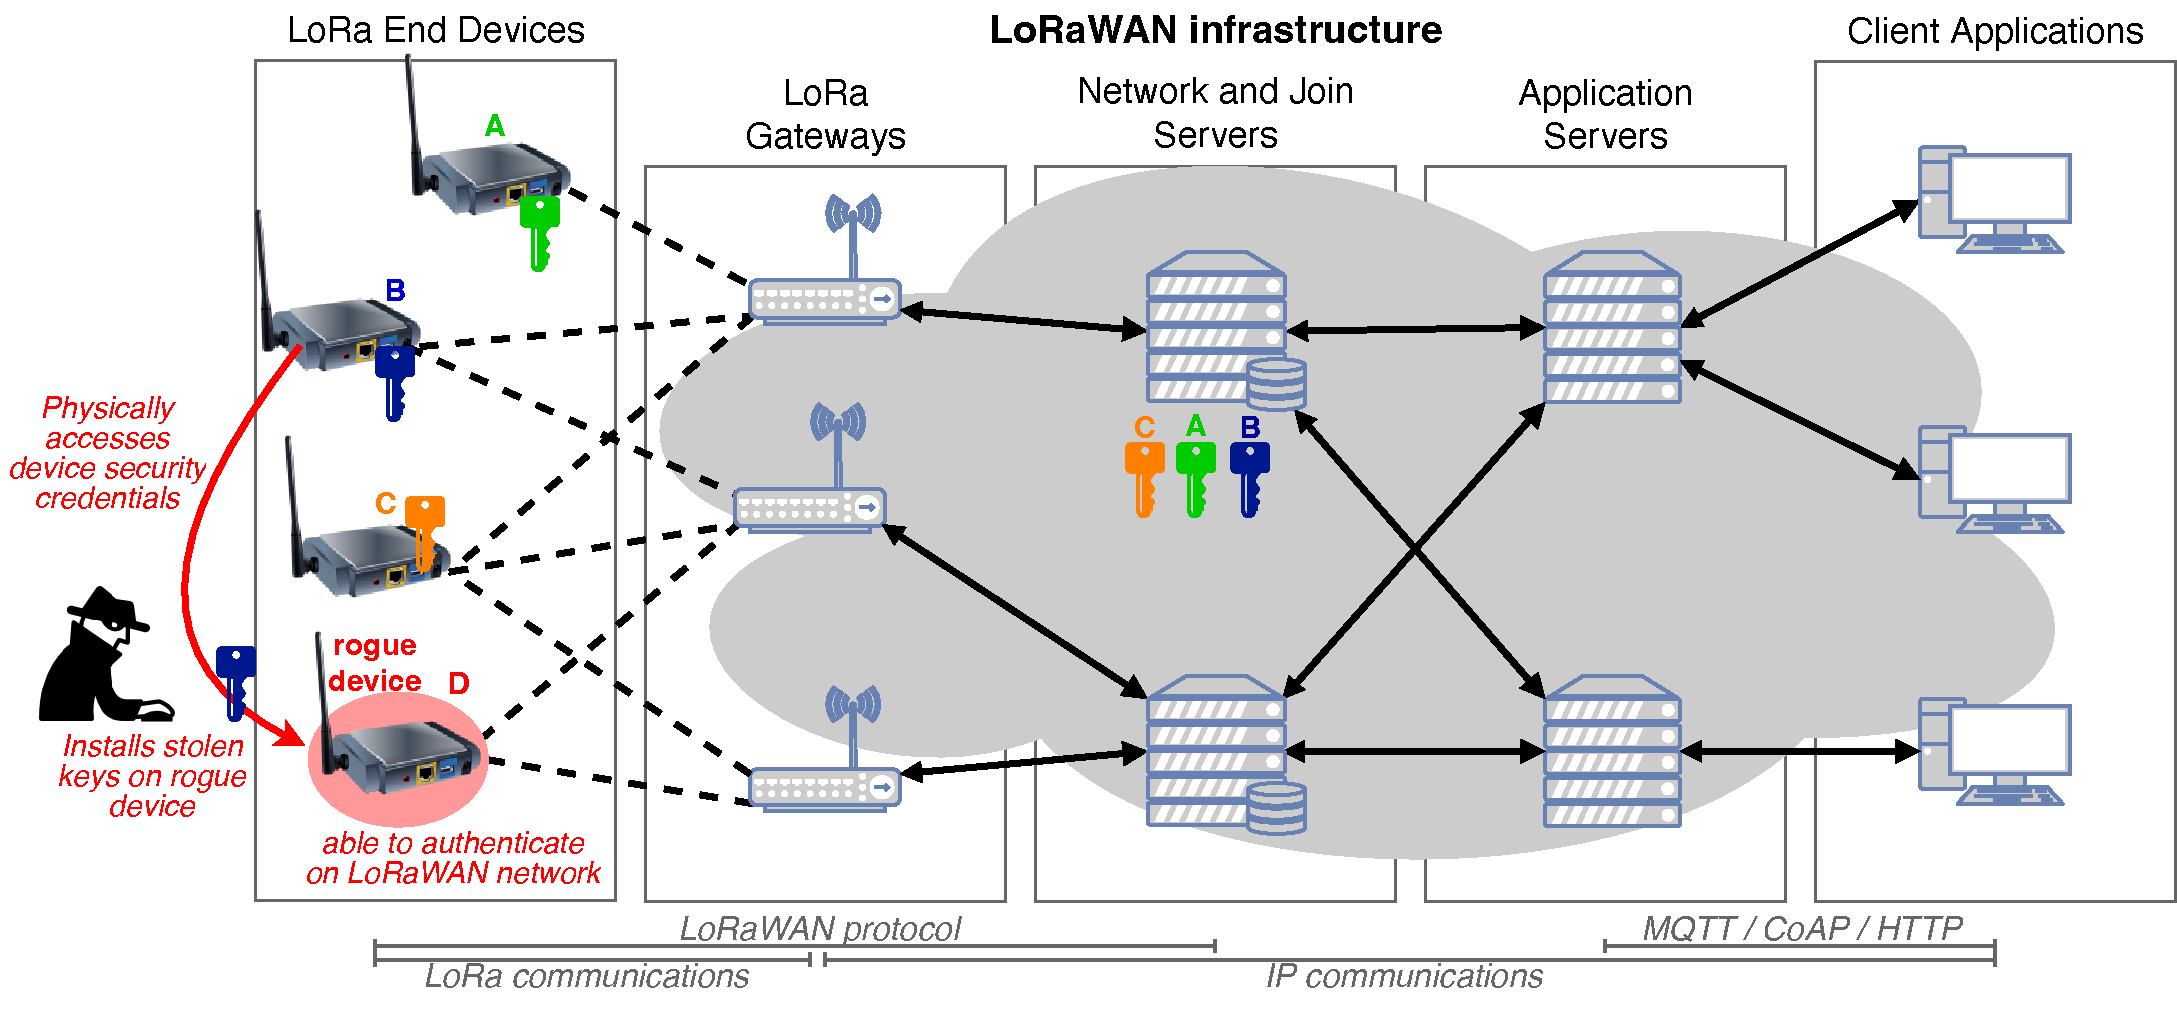
\includegraphics[width=0.95\textwidth]{figures/LoRaWAN2.pdf}
    \end{center}
  \end{figure}
\end{frame}

\begin{frame}
  \frametitle{LoRa physical layer}
  \small
  LoRa physical layer is based on Chirp Spread Spectrum (CSS) modulation. 


  \begin{definition}[Chirp Spread Spectrum modulation]
    CSS modulation is based on sine signals whose frequency varies linearly over time.
  \end{definition}

  \begin{figure}
    \begin{center}
      \includesvg[width=0.95\textwidth]{figures/timeVsFreq.svg}
    \end{center}
    \caption{Time vs Frequency Domain of a LoRa up-chirp}
  \end{figure}
\end{frame}

\begin{frame}
  \frametitle{LoRa frame}

  The LoRa frame is composed of :
  \begin{enumerate}
    \item A preamble (8 up-chirps and Sync word)
    \item A Start of Frame Delimiter (SFD)
    \item A payload
  \end{enumerate}

  \begin{figure}
    \begin{center}
      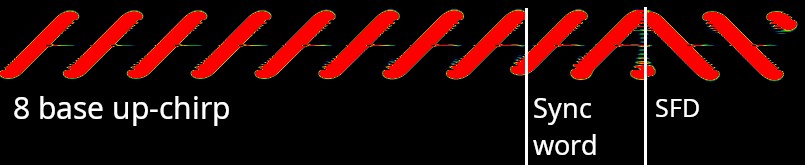
\includegraphics[width=0.95\textwidth]{figures/LoRaPreambleWithText.png}
    \end{center}
    \caption{Preamble and SFD parts on a spectrogram}
  \end{figure}
\end{frame}


\subsection{Radio frequency fingerprinting identification}
\begin{frame}
  \frametitle{RFFI}
  \begin{definition}{Radio Frequency Fingerprints (RFF)}
    are subtle impairments in a device transmission due to its hardware components. 
 \end{definition}
 \pause

 RFF are unique to each device which makes it a key candidate for device authentication.
  
 \pause

  \begin{definition}{Radio Frequency Fingerprinting Identification (RFFI)}
    bases Identification on the RFF of a device. 
 \end{definition}

\end{frame}

\subsection{State of the art}
\begin{frame}
  \frametitle{State of the art}
  Recent studies\footnotemark  have looked into LoRa RFFI with DL models.

  However, as stated by Aqeel in a recent survey\footnotemark , only four datasets are publicly available. 
  \begin{enumerate}
    \item Zenodo 
    \item Oregon state University cloud 
    \item IEEE dataport (2)  
  \end{enumerate}


  \footnotetext[1]{\cite{shen2021radio} and \cite{al2021deeplora}}
  \footnotetext[2]{\cite{AqeelSurvey}}


\end{frame}

\subsection{Objective}
\begin{frame}
  \frametitle{Objective}
  
  The Goals of this internship were to:
  \begin{enumerate}
      \item Understand the principles of LoRa technology
      \item Establish a test bed scenario to collect LoRa radio frequency signals
      \item Collect LoRa RF signals at different distances to evaluate the impact on DL classification
  \end{enumerate}
  
\end{frame}


%%%%%%%%%%%%%%%%%%%%%%%%%%%%%%%%%%%%%%%%%%%%
% appendix

 % methodology part 

% present hardware setup
% Rx side photo : yes
% Tx side photo : on the way 
% discuss synchro methods 
% ? discuss demod ?  => let in appendix ?
% Comparaison and selection


\section{Methodology}
\subsection{Experimental setup}
\begin{frame}
  \only<1>{
  \frametitle{Experimental setup}
  \begin{figure}
    \begin{center}
      \includesvg[width=0.95\textwidth]{figures/layout1.svg}
    \end{center}
    \caption{Setup schematic}
  \end{figure}}

  \only<2>{
  \frametitle{Experimental setup}
  \begin{figure}
    \begin{center}
      \includesvg[width=0.95\textwidth]{figures/layout2.svg}
    \end{center}
    \caption{Setup schematic}
  \end{figure}}


  \only<3>{
  \frametitle{Experimental setup}
  \begin{figure}
    \begin{center}
      \includesvg[width=0.95\textwidth]{figures/layout3.svg}
    \end{center}
    \caption{Setup schematic}
\end{figure}}

  \only<4>{
  \frametitle{Experimental setup}
  \begin{figure}
    \begin{center}
      \includesvg[width=0.95\textwidth]{figures/layout4.svg}
    \end{center}
    \caption{Setup schematic}
  \end{figure}}

\end{frame}


\begin{frame}
  \frametitle{Transmitter side in photo}
  \begin{figure}[ht]
  \begin{adjustwidth}{-10cm}{-10cm}
    \centering
    \begin{subfigure}[ht]{0.5\textwidth}
      \centering
      \includegraphics[width=\textwidth, angle=270]{figures/Tx.jpg}
      \caption{front view}
    \end{subfigure}
    \begin{subfigure}[ht]{0.5\textwidth}
      \centering
      \includegraphics[width=\textwidth, angle=270]{figures/Txpov.jpg}
      \caption{receiver side point of view}
    \end{subfigure}

    \caption{Transmitter side views}
    \end{adjustwidth}
  \end{figure}
\end{frame}


\begin{frame}
  \frametitle{Receiver side in photo}

  \begin{figure}[ht]
  \begin{adjustwidth}{-10cm}{-10cm}
    \centering
    \begin{subfigure}[ht]{0.5\textwidth}
      \centering
      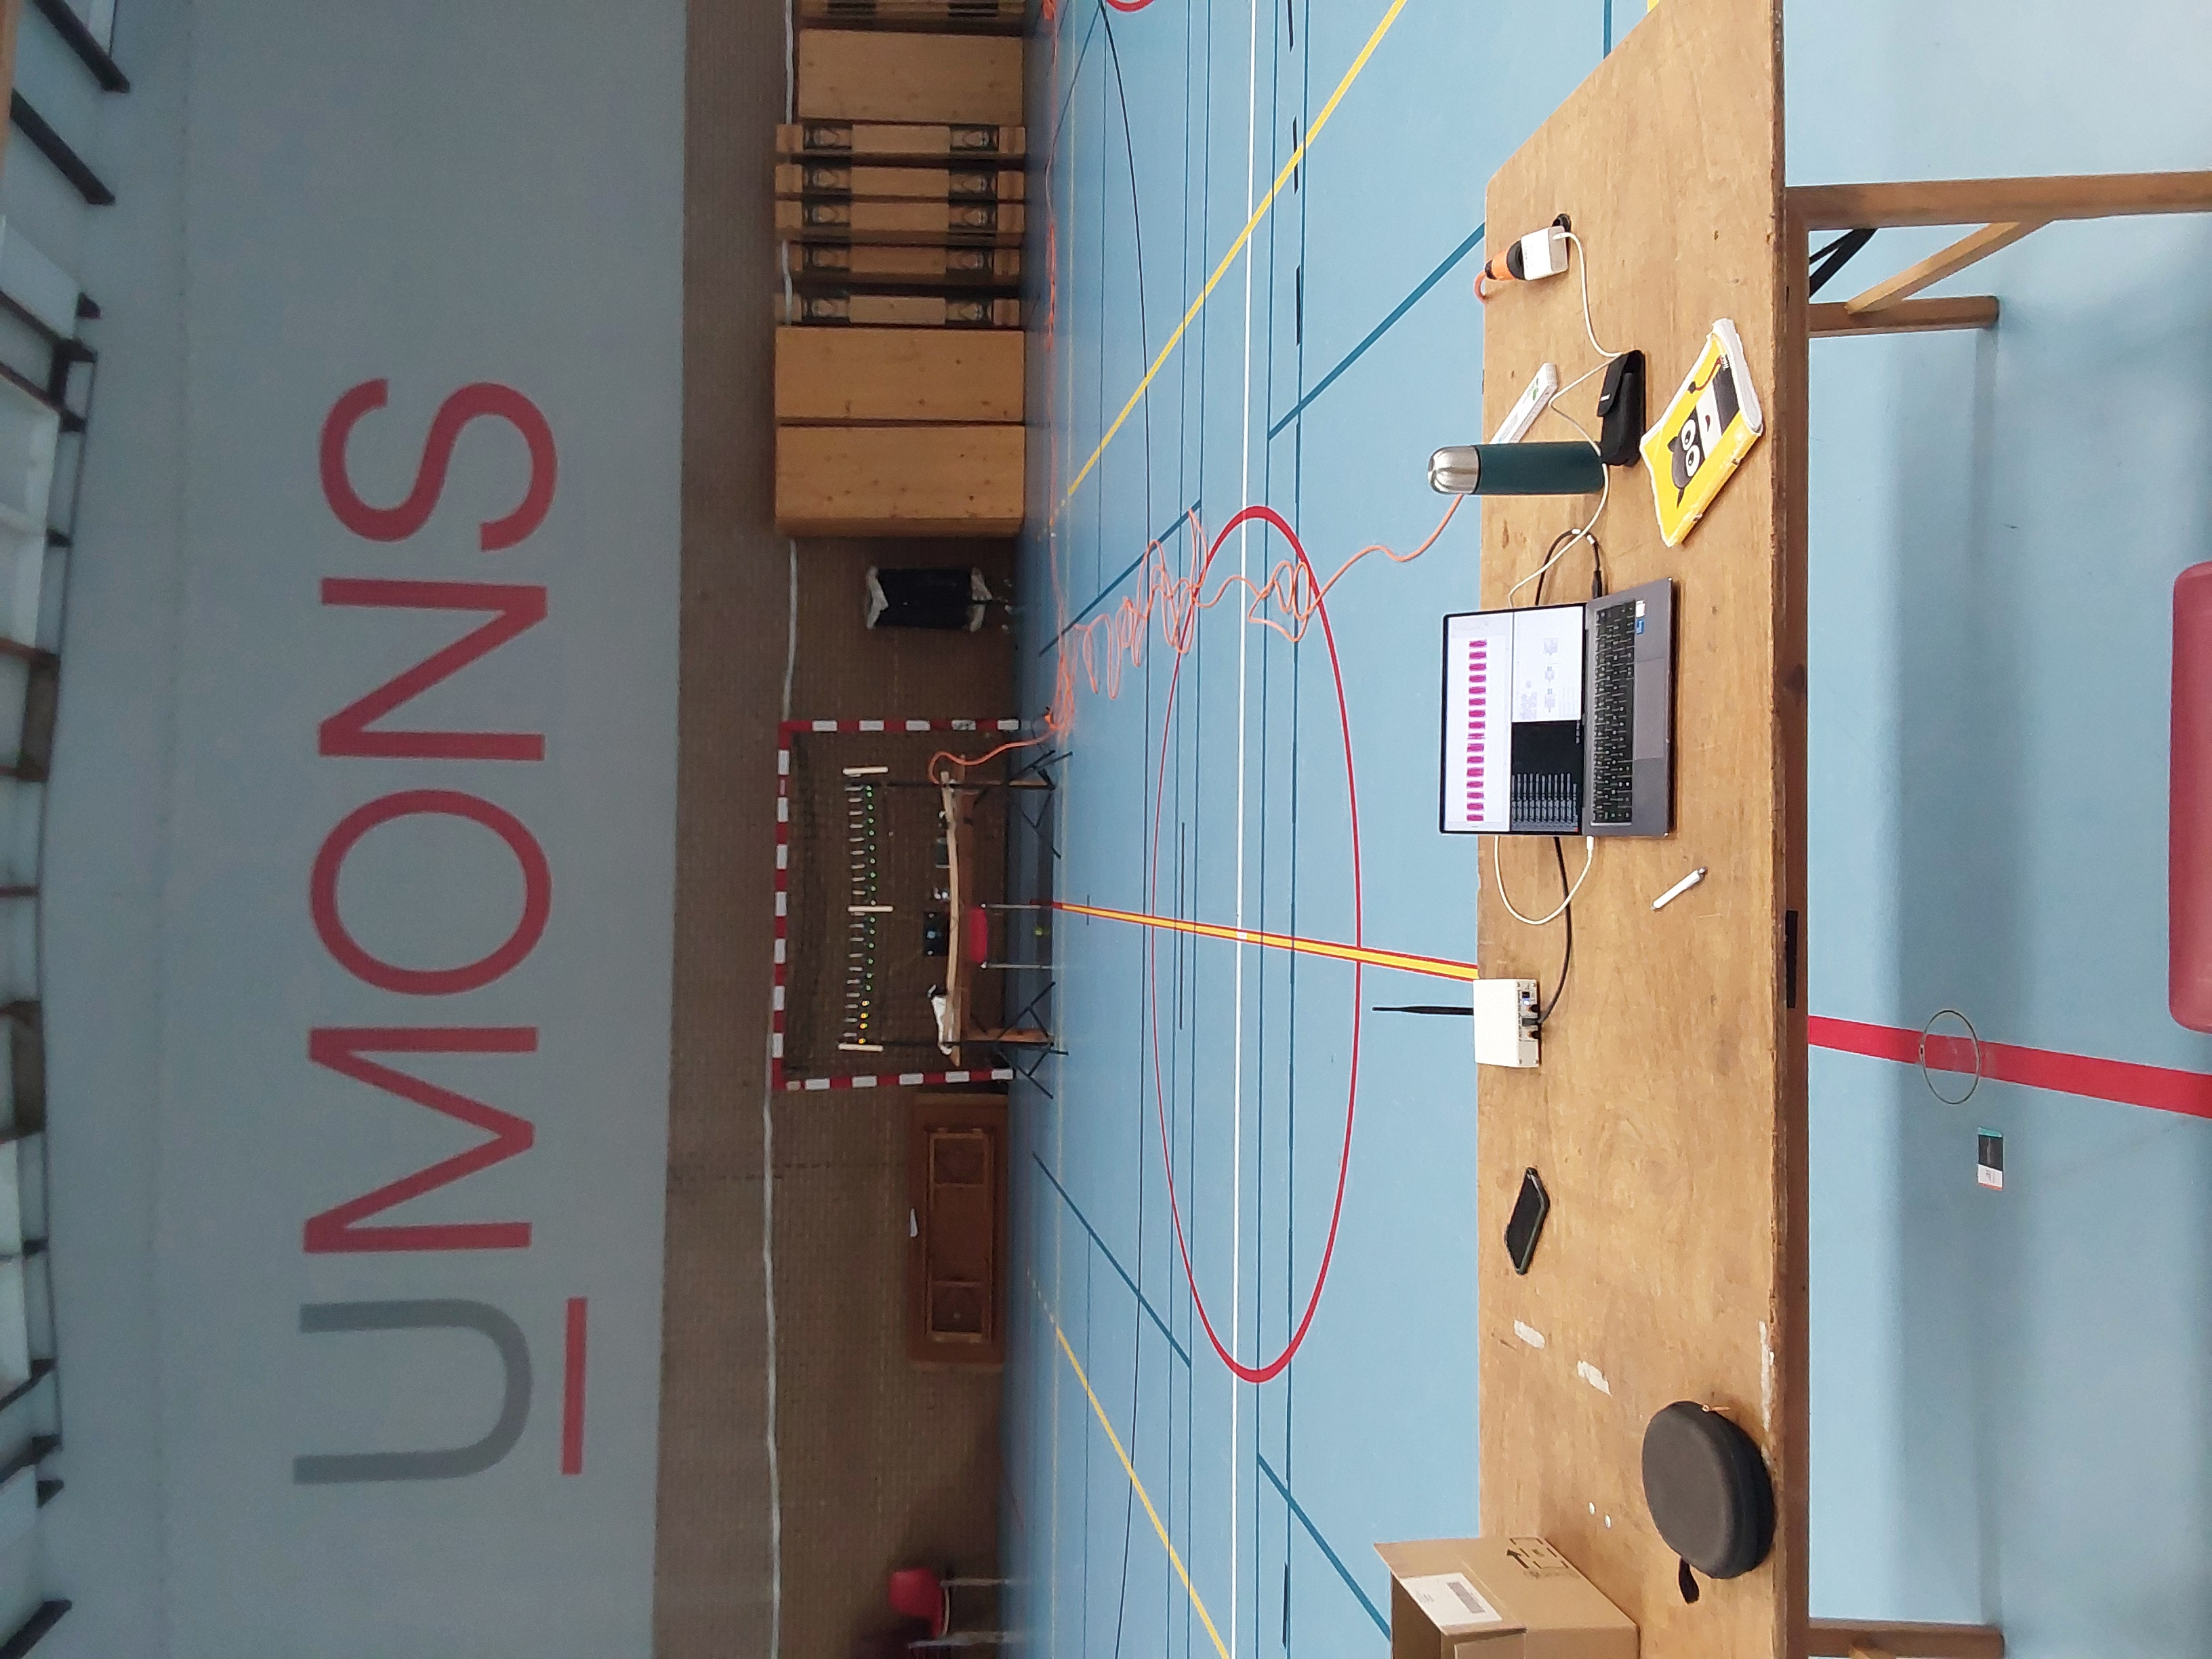
\includegraphics[width=\textwidth, angle=270]{figures/inside rx.jpg}
      \caption{Indoors scenario}
    \end{subfigure}
    \begin{subfigure}[ht]{0.5\textwidth}
      \centering
      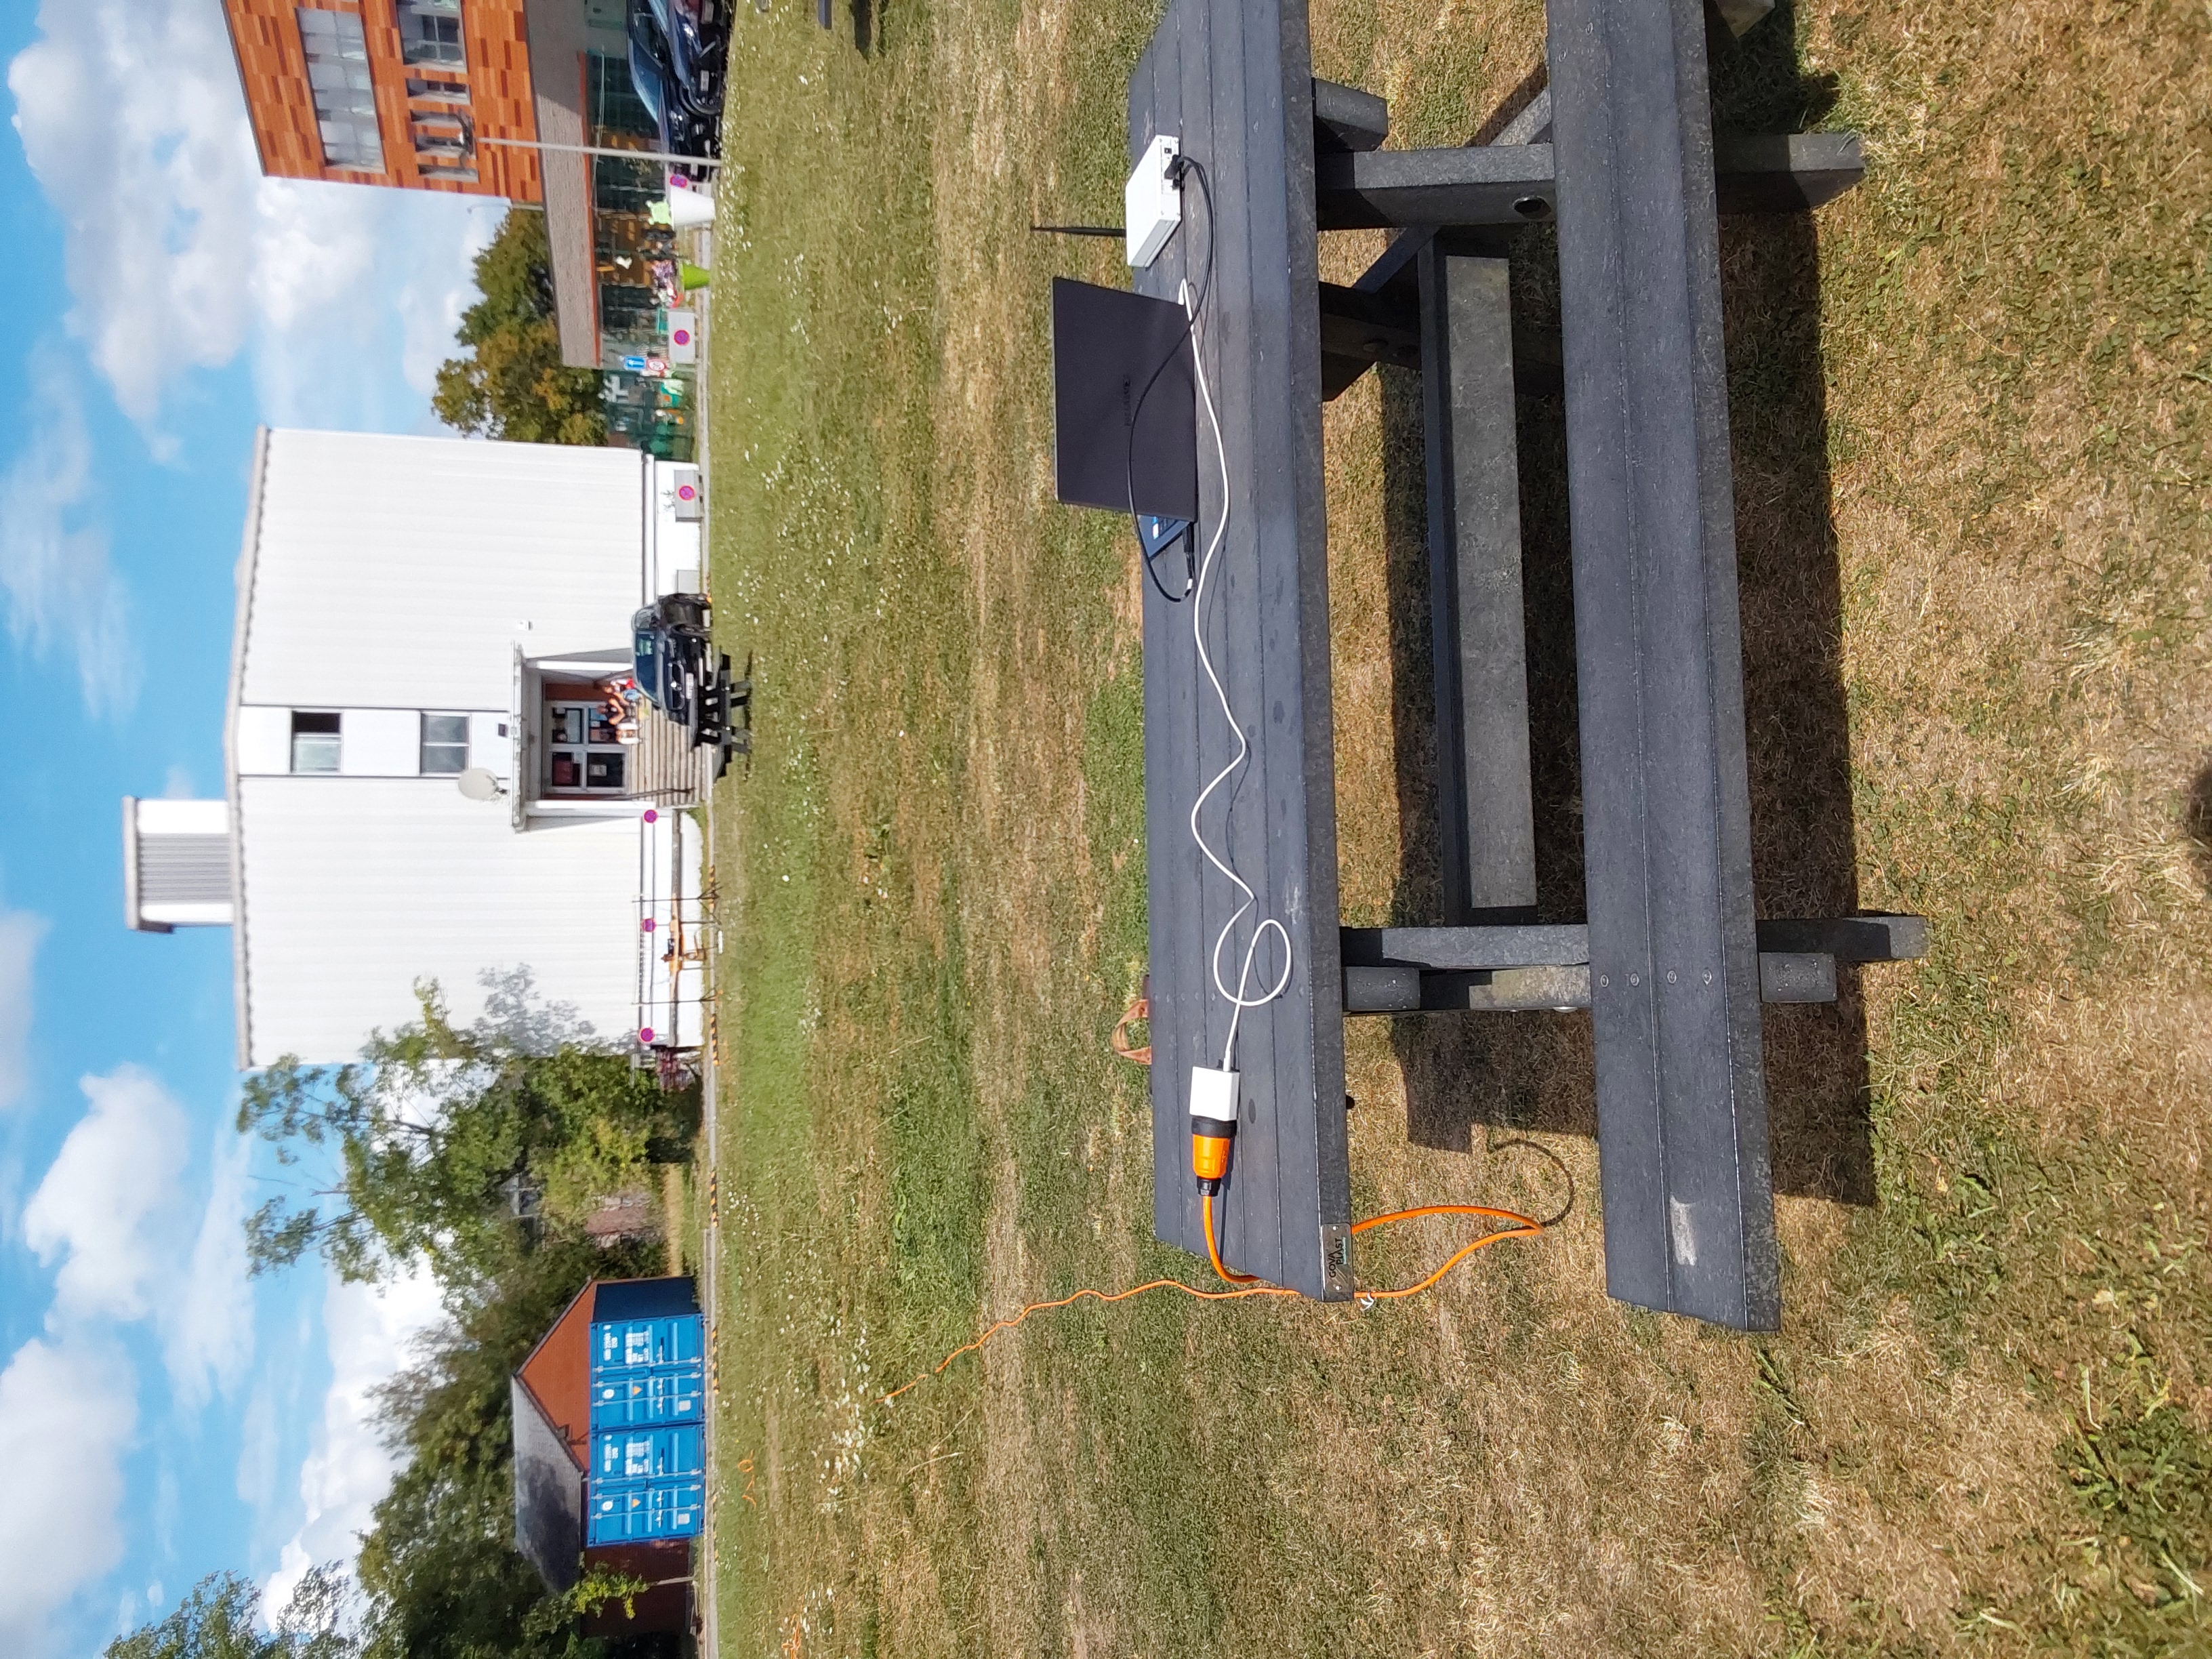
\includegraphics[width=\textwidth, angle=270]{figures/outside rx.jpg}
      \caption{Outdoors scenario}
    \end{subfigure}

    \caption{Receiver side indoors and outdoors}
    \end{adjustwidth}
  \end{figure}
\end{frame}



\subsection{Transmission methods}
\begin{frame}
  \frametitle{Transmission methods}
  \only<2>{
  \textbf{Round Robin (RR) }: each device sends a frame then passes the turn to the next one. The last device passes the turn to the first one. \\ }

  \only<3>{
  \textbf{One by One (ObO)}: each device sends all its frames then passes the turn to the next one.}

  \begin{figure}[ht]
  \begin{adjustwidth}{-10cm}{-10cm}
    \centering

  \only<2>{
    \begin{subfigure}[ht]{0.5\textwidth}
      \centering
      \includesvg[width=0.98\textwidth]{figures/RR.svg}
      \caption{RR method}
    \end{subfigure}
  }
  \only<3>{
    \begin{subfigure}[ht]{0.5\textwidth}
      \centering
      \includesvg[width=\textwidth]{figures/ObO.svg}
      \caption{ObO method}
    \end{subfigure}
  }
    \end{adjustwidth}
  \end{figure}

\end{frame}


\begin{frame}
  \frametitle{Comparison properties}
  The most important properties to compare those methods are :
  \begin{enumerate}
    \item Quality : How little the scheduling impacts the DL classification
    \item Safety : At any point, the receiver has to be certain of the origin of a LoRa frame
  \end{enumerate}

\end{frame}

\begin{frame}
  \frametitle{Selection}

  \only<2>{
  \begin{figure}
    \begin{center}
      \includesvg[width=0.90\textwidth]{figures/temp1.svg}
    \end{center}
  \end{figure}}

  \only<3>{
  \begin{figure}
    \begin{center}
      \includesvg[width=0.90\textwidth]{figures/temp2.svg}
    \end{center}
  \end{figure}}

  \only<4>{
  \begin{figure}
    \begin{center}
      \includesvg[width=0.90\textwidth]{figures/temp3.svg}
    \end{center}
  \end{figure}}

  \only<5>{
  \begin{figure}
    \begin{center}
      \includesvg[width=0.80\textwidth]{figures/temp3.svg}
    \end{center}
  \end{figure}}

  \only<5>{
  Even thought quality is an important property, safety is mandatory.\\ 
  \hspace{1cm}
   
  Because misclassification can occur when a device passes its turn, to avoid any misclassification by the receiver, the One by One method was selected. }
\end{frame}
  




\section{Results analysis}
\subsection{Data exploratory analysis}

\begin{frame}
  \frametitle{Time domain over distance}
  \begin{figure}
    \begin{center}
      \includesvg[width=0.8\textwidth]{figures/2Vs8chirps.svg}
    \end{center}
    \caption{Captured signals}
  \end{figure}
\end{frame}

\begin{frame}
  \frametitle{Time domain over distance}
  \begin{figure}
    \begin{center}
      \includesvg[width=0.8\textwidth]{figures/20deviceTimeDomtimeplot.svg}
    \end{center}
    \caption{Signals of the $20^{th}$ device indoor in the time domain}
  \end{figure}
\end{frame}

\begin{frame}
  \frametitle{Histograms}
  \begin{figure}
    \begin{center}
      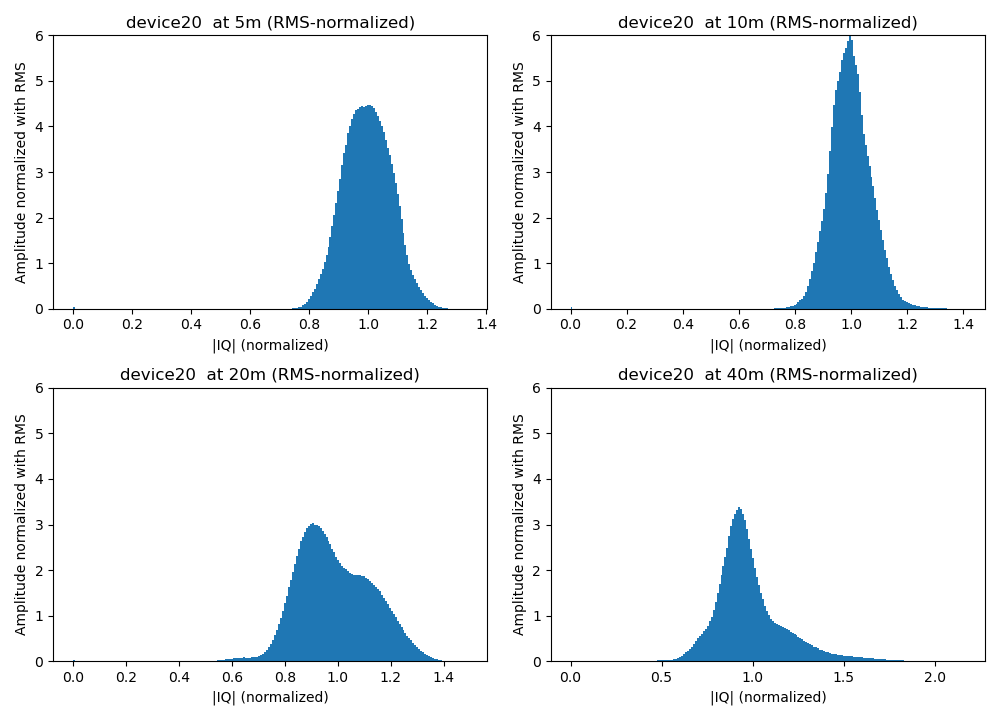
\includegraphics[width=0.75\textwidth]{figures/histo.png}
    \end{center}
    \caption{Histograms of the $20^{th}$ device at different distances Indoor}
  \end{figure}
\end{frame}

\subsection{Problem encountered}

\begin{frame}
  \only<1>{
  \frametitle{Problem encountered}
  \begin{enumerate}
    \item Power supply
    \item Arduino communications
    \item Synchronizing the capture 
    \item Double captures
  \end{enumerate}}

  \only<2>{
  \frametitle{Problem encountered}
  \begin{enumerate}
    \item \sout{Power supply}
    \item \sout{Arduino communications}
    \item \sout{Synchronizing the capture}
    \item Double captures
  \end{enumerate}}
\end{frame}


\begin{frame}
  \frametitle{Problem encountered}
  \begin{definition}
   A double capture is a capture containing 2 frames instead of one.
  \end{definition}
  \pause

  \begin{figure}[ht]
  \begin{adjustwidth}{-10cm}{-10cm}
    \centering
    \begin{subfigure}[ht]{0.47\textwidth}
      \centering
      \includesvg[width=\textwidth]{figures/normalcap.svg}
      \caption{normal capture scheme}
    \end{subfigure}
    \pause
    \begin{subfigure}[ht]{0.47\textwidth}
      \centering
      \includesvg[width=\textwidth]{figures/doublecap.svg}
      \caption{double capture scheme}
    \end{subfigure}
  \end{adjustwidth}
  \end{figure}
  

\end{frame}

% \begin{frame}
%   \frametitle{Results table Indoors}
%   \begin{table}[ht]
%     \small
%     \caption{Frames Captured Indoors. The total number of frames is presented. In parentheses is the number of double captures}
%     \centering
%       \resizebox{0.488\linewidth}{!}{%
%       \begin{tabular}{|c|c|c|c|c|c|}
%         \hline
%         \multicolumn{6}{|c|}{\textbf{Frames Captured indoor}} \\
%         \hline
%         \textbf{device ID} & \textbf{5\unit{\m}} & \textbf{10\unit{\m}} & \textbf{20\unit{\m}} & \textbf{30\unit{\m}} & \textbf{40\unit{\m}} \\
%         \hline
%         1& 539(0)&544(1)&541(0)&520(0)&537(0)
%         \\ \hline
%         2& 526(0)&542(0)&526(25)&530(0)&532(0)
%         \\ \hline
%         3& 543(0)&540(1)&541(121)&539(0)&535(0)
%         \\ \hline
%         4& 531(0)&528(0)&532(93)&530(1)&535(0)
%         \\ \hline
%         5& 533(0)&530(0)&531(52)&532(2)&536(0)
%         \\ \hline
%         6& 523(0)&531(1)&533(23)&527(4)&522(0)
%         \\ \hline
%         7& 533(0)&539(3)&544(20)&544(8)&540(0)
%         \\ \hline
%         8& 534(0)&530(9)&535(12)&542(22)&541(0)
%         \\ \hline
%         9& 542(0)&542(49)&530(14)&541(21)&540(0)
%         \\ \hline
%         10& 543(0)&543(47)&536(11)&541(28)&543(0)
%         \\ \hline
%         11& 540(0)&537(0)&542(11)&533(44)&533(0)
%         \\ \hline
%         12& 537(0)&539(0)&524(8)&533(48)&537(0)
%         \\ \hline
%         13& 525(0)&533(0)&534(4)&534(84)&527(0)
%         \\ \hline
%         14& 538(0)&535(0)&528(6)&539(102)&534(0)
%         \\ \hline
%         15& 524(0)&540(0)&509(3)&533(126)&519(0)
%         \\ \hline
%         16& 534(0)&537(0)&528(3)&535(130)&538(0)
%         \\ \hline
%         17& 541(0)&537(0)&531(3)&538(124)&526(0)
%         \\ \hline
%         18& 532(0)&535(0)&535(1)&533(132)&529(0)
%         \\ \hline
%         19& 538(0)&542(0)&541(3)&542(133)&540(1)
%         \\ \hline
%         20& 536(0)&534(0)&535(2)&537(112)&531(0)
%         \\ \hline
%         \hline
%         \textbf{total} & 10692&10738&10656&10703&10675\\ 
%         \hline
%     \end{tabular}}%
%   \end{table}
%   % two important observation : not less detection with increasing distance and the double captures
% \end{frame}
%
%
%
% \begin{frame}
%   \frametitle{Results table Outdoors}
% \begin{table}[H]
%     \small
%
%     \caption{Frames Captured Outdoors. The total number of frames is presented. In parentheses is the number of double captures}
%   \centering
%       \resizebox{0.577\linewidth}{!}{%
%     \begin{tabular}{|c|c|c|c|c|c|c|}
%       \hline
%       \multicolumn{7}{|c|}{\textbf{Frames Captured outdoor}} \\
%       \hline
%       \textbf{device ID} & \textbf{5\unit{\m}} & \textbf{10\unit{\m}} & \textbf{20\unit{\m}} & \textbf{30\unit{\m}} & \textbf{40\unit{\m}} & \textbf{50\unit{\m}}\\
%       \hline
% 1& 520(95)&538(26)&532(2)&523(0)&535(56)&540(71)
% \\ \hline
% 2& 531(124)&535(64)&532(18)&534(1)&534(32)&536(59)
% \\ \hline
% 3& 534(37)&542(0)&536(7)&538(1)&536(10)&545(37)
% \\ \hline
% 4& 532(2)&525(1)&532(1)&533(4)&535(12)&531(28)
% \\ \hline
% 5& 466(0)&538(1)&537(3)&534(53)&538(45)&540(54)
% \\ \hline
% 6& 517(0)&535(0)&533(67)&535(3)&529(76)&536(7)
% \\ \hline
% 7& 530(2)&530(1)&533(16)&547(1)&541(44)&532(0)
% \\ \hline
% 8& 482(0)&520(63)&523(3)&533(89)&536(13)&529(0)
% \\ \hline
% 9& 514(1)&520(51)&537(2)&540(25)&540(0)&523(0)
% \\ \hline
% 10& 528(1)&530(1)&541(8)&532(0)&541(0)&526(3)
% \\ \hline
% 11& 476(1)&524(0)&541(2)&526(1)&546(0)&521(2)
% \\ \hline
% 12& 505(0)&519(1)&539(2)&525(0)&542(4)&533(2)
% \\ \hline
% 13& 508(1)&529(2)&528(0)&529(5)&535(6)&536(1)
% \\ \hline
% 14& 476(63)&539(52)&541(2)&533(0)&537(5)&540(0)
% \\ \hline
% 15& 503(47)&529(28)&542(3)&484(0)&530(1)&516(0)
% \\ \hline
% 16& 529(11)&540(16)&532(1)&523(0)&533(96)&526(1)
% \\ \hline
% 17& 527(2)&538(9)&530(5)&527(3)&537(55)&535(48)
% \\ \hline
% 18& 529(2)&531(8)&529(8)&520(3)&540(1)&525(77)
% \\ \hline
% 19& 526(2)&536(13)&540(1)&535(5)&545(3)&534(20)
% \\ \hline
% 20& 527(1)&541(14)&530(27)&532(13)&539(0)&536(0)
% \\ \hline
%       \hline
%       \textbf{total} & 10260&10639&10688&10583&10749&10640 \\
%       \hline
%   \end{tabular}}
% \end{table}
% \end{frame}





\section{Conclusion}

\begin{frame}
  \frametitle{Conclusion}
  \textbf{In conclusion, during this internship :}
  \begin{enumerate}
    \item We established a stable experimental setup 
    \item We successfully collected 2 datasets with varying distance
    \item I learned signal processing basics with LoRaPHY
  \end{enumerate}

  \pause


  \textbf{Future Improvements :}
  \begin{enumerate}
    \item Try to use an Ethernet cable instead of a mobile hotspot 
    \item Try to use a single laptop as receiver and transmitter 
    \item Make the Round robin method reliable
    \item And... Document my code properly !
  \end{enumerate}
\end{frame}

\begin{frame}

  \centering
  \huge Thank you for listening
  
\end{frame}


\printbibliography

\end{document}
